\documentclass[xetex]{beamer}

\usepackage{xltxtra}
\usepackage{xcolor}
\usepackage{pgfplots}

\usetheme{Rochester}
\beamertemplatenavigationsymbolsempty

\title{cuRAND}
\author{Dányi Bence\\ Kálmán Viktor}

\begin{document}
  \frame{\titlepage}
  \begin{frame}
    \frametitle{CUDA}
    \framesubtitle{Bevezető}
    \begin{itemize}
      \item Párhuzamos feldolgozás platform és programozási modell
      \item GPGPU
      \pause
      \item Alacsony és magas szintű API
        \begin{itemize}
          \item CUDA driver API
          \item CUDA runtime API
        \end{itemize}
    \end{itemize}

    \begin{center}
      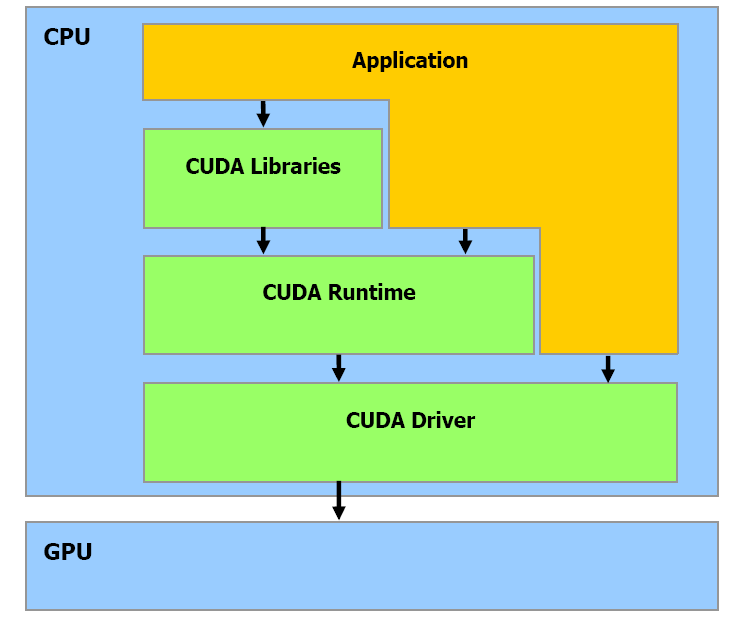
\includegraphics[width=0.5\textwidth]{figures/cudapi.png}
    \end{center}
  \end{frame}
  \begin{frame}
    \frametitle{CUDA}
    \framesubtitle{Bevezető}
    \begin{itemize}
      \item C, C++, Fortran támogatás
      \item Saját LLVM alapú fordító (nvcc)
      \item Python (PyCUDA), Perl, Java, Ruby wrapper
      \item Rengeteg könyvtár: cuDNN (neurális hálók), cuFFT, nvGRAPH, FFmpeg, cuBLAS
    \end{itemize}

  \end{frame}
  \begin{frame}
    \frametitle{CUDA}
    \framesubtitle{Negatívumok}
    \begin{itemize}
      \item C++-ként fordít -> valid C, de nem valid C++ elhasal
      \item Nincs kivételkezelés
      \item Host és device közötti másolgatás
      \item Csak NVIDIA
    \end{itemize}
  \end{frame}
  \begin{frame}
    \frametitle{CUDA}
    \framesubtitle{Workflow}
    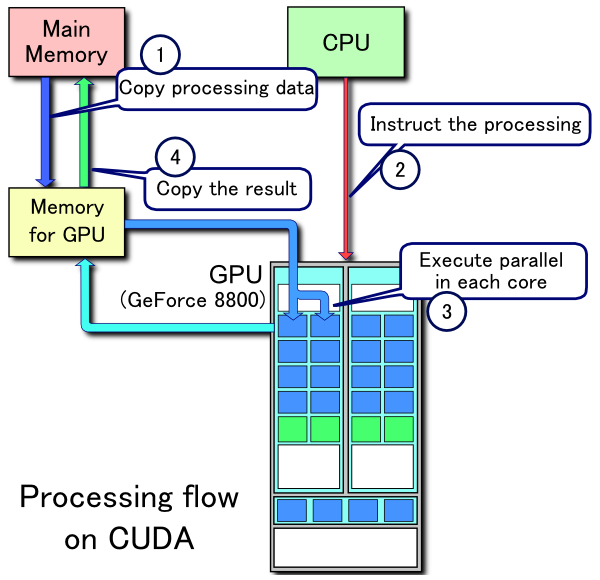
\includegraphics[width=10cm]{figures/cuda_workflow.png}
  \end{frame}
  \begin{frame}
    \frametitle{cuRAND}
    A cuRAND könyvtár az NVIDIA megoldása véletlen számok generálására
    \begin{itemize}
      \item Host API
      \item Device API
      \item kb 9 féle generátor
      \item Pszeudorandom sorozat: statisztikailag véletlen számok
      \item Kvázirandom sorozat (alacsony diszkrepanciájú): egy $n$-dimenziós teret egyenletesen töltenek ki
      \item Egyenletes/normál/poisson/stb eloszlás
    \end{itemize}
  \end{frame}
  \begin{frame}
    \frametitle{Host API}
    A cuRAND API hívható hoszt környezetben is
    \begin{itemize}
      \item $n$ szám generálása (párhuzamosan)
      \item fallback CPU generátorra, ha nem érhető el CUDA
      \item minden szükséges paraméter egy \texttt{curandGenerator\_t}-ben
    \end{itemize}
  \end{frame}
  \begin{frame}
    \frametitle{Használat}
    \begin{itemize}
      \item \texttt{curandCreateGenerator(*gen, type)}
      \item Host memória foglalás \texttt{malloc(size)}
      \item Device memória foglalás \texttt{cudaMalloc(**p, size)}
      \item Inicializálás
        \begin{itemize}
          \item \texttt{curandSetPseudoRandomGeneratorSeed(gen, seed)}
          \item \texttt{curandSetQuasiRandomGeneratorDimensions(gen, dimensions)}
        \end{itemize}
      \item Generálás
      \begin{itemize}
        \item \texttt{curandGenerate*(gen, *out, n)}
      \end{itemize}
      \item Eredmény visszamásolása host memóriába: \texttt{cudaMemcpy(*to, *from, size, cudaMemcpyDeviceToHost)}
    \end{itemize}
  \end{frame}
  \begin{frame}
    \frametitle{Device API}
    Device API hívható CUDA kernelel belül (\texttt{my\_kernel<<<blocks, threads>>>(...)})
    \begin{itemize}
      \item $1$ elem generálása hívásonként
      \item Generátor állapot: \texttt{*curandState}
      \item Minden szál saját állapottal rendelkezik (\texttt{curandState} tömb)
    \end{itemize}
  \end{frame}
  \begin{frame}
    \frametitle{Használat}
    \begin{itemize}
      \item Memória foglalás az állapotnak: \texttt{cudaMalloc(**p, size)}
      \item Memória foglalás az eredménynek: \texttt{cudaMalloc(**p, size)}
      \item Memória foglalás az eredménynek (host): \texttt{malloc(size)}
      \item Inicializálás (kernelen belül): \texttt{curand\_init(seed, seq, offset, *state)}
      \item Generálás (kernelen belül): \texttt{curand\_*(*state)}
      \item Eredmény visszamásolása: \texttt{cudaMemcpy(*to, *from, size, cudaMemcpyDeviceToHost)}
    \end{itemize}
  \end{frame}
  \begin{frame}
    \frametitle{Pszeudorandom sorozat}
    \begin{tikzpicture}
      \begin{axis}[scatter/classes={a={mark=o,draw=black}}]
        \addplot[scatter,only marks,scatter src=explicit symbolic,row sep=crcr] table[meta=label,col sep=comma] {pseudo-points.csv};
      \end{axis}
    \end{tikzpicture}
  \end{frame}
  \begin{frame}
    \frametitle{Alacsony diszkrepanciás sorozat}
    \begin{tikzpicture}
      \begin{axis}[scatter/classes={a={mark=o,draw=black}}]
        \addplot[scatter,only marks,scatter src=explicit symbolic,row sep=crcr] table[meta=label,col sep=comma] {quasi-points.csv};
      \end{axis}
    \end{tikzpicture}
  \end{frame}
  \begin{frame}
    \frametitle{Egyenletes eloszlás}
    \begin{tikzpicture}
      \begin{axis}[ymin=0,ymax=200000,enlargelimits=false,xmin=0,xmax=100]
        \addplot table[col sep=comma] {uniform-hist.csv};
      \end{axis}
    \end{tikzpicture}
  \end{frame}
  \begin{frame}
    \frametitle{Normál eloszlás}
    \begin{tikzpicture}
      \begin{axis}
        \addplot table[col sep=comma] {normal-hist.csv};
      \end{axis}
    \end{tikzpicture}
  \end{frame}
  \begin{frame}
    \frametitle{CUDA vs Intel MKL}
    \framesubtitle{Összehasonlítás}
    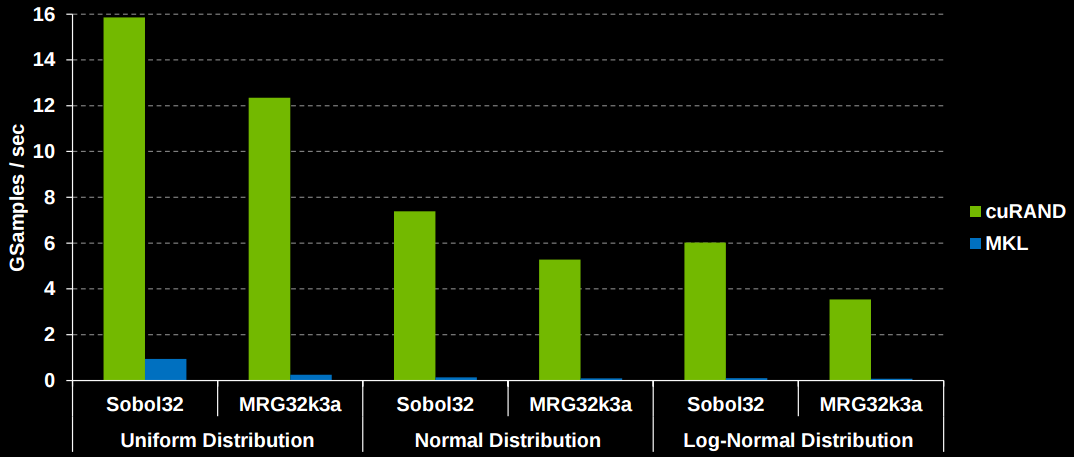
\includegraphics[width=1.0\textwidth]{figures/cuda_vs_mkl.png}
    \\
    \pause
    \begin{center}
      NVIDIA Tesla K40M (2880 CUDA cores) \\
      vs \\
      Intel Xeon E5-2698 (16 cores @ 3.6 Ghz)
    \end{center}
  \end{frame}
  \begin{frame}
    \frametitle{CUDA vs Intel MKL}
    \framesubtitle{Emberközelibb összehasonlítás}
    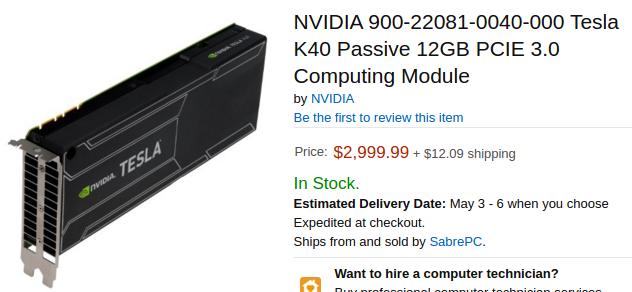
\includegraphics[width=1.0\textwidth]{figures/tesla.png}
  \end{frame}
  \begin{frame}
    \frametitle{CUDA vs Intel MKL}
    \framesubtitle{Emberközelibb összehasonlítás}
    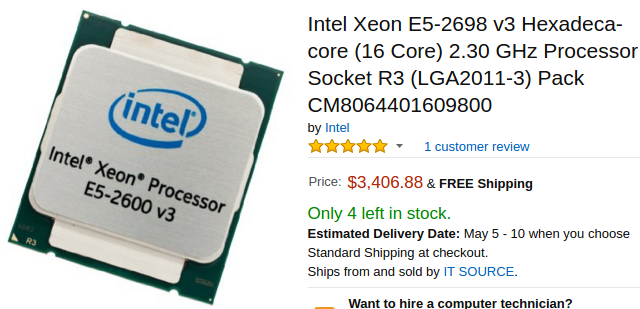
\includegraphics[width=1.0\textwidth]{figures/xeon.png}
  \end{frame}
\end{document}
